\documentclass[9pt]{beamer}

\usetheme{metropolis}
\usepackage{appendixnumberbeamer}

\usepackage{booktabs}
\usepackage[scale=2]{ccicons}


\usepackage{tikz}
\usetikzlibrary{shapes,arrows}
\usepackage{amsmath, bm}
\usepackage{physics}
\usepackage{mathtools}

\usepackage{pgfplots}
\usepgfplotslibrary{dateplot}

\usepackage{xspace}
\usepackage{soul}
\newcommand{\themename}{\textbf{\textsc{metropolis}}\xspace}

\DeclareMathOperator{\msbar}{\overline{MS}}
\DeclareMathOperator{\dis}{DIS}
\DeclareMathOperator{\phys}{PHYS}
\DeclareMathOperator{\pos}{POS}
\DeclareMathOperator{\dpos}{DPOS}
\DeclareMathOperator{\mpos}{MPOS}

\title{Can $\msbar$ PDF be negative?}
%\subtitle{make PDFs positive and everyone happy}
\date{February, 2020}
\author{Alessandro Candido
}
%\institute{N3PDF}
\titlegraphic{
%        \raisebox{5pt}[0pt][0pt]{
\includegraphics[height=0.8cm]{../_logos/nnpdf_logo.pdf}}\hspace*{10pt}
        \hfill
        \raisebox{5pt}[0pt][0pt]{
\includegraphics[height=0.8cm]{../_logos/n3pdf_logo.pdf}}\hspace*{10pt}
        
\includegraphics[height=1.3cm]{../_logos/erc_logo1.png}

        \vfill\vspace*{170pt}
        
\includegraphics[height=1cm]{../_logos/unimi_logo.png}\hfill
        
\includegraphics[height=1cm]{../_logos/infn_logo.png}\\
        \vspace*{5pt}
        {\fontsize{3pt}{3.5pt}\selectfont
             \begin{center}
                 This project has received funding from the European Union's Horizon 2020 research and innovation programme under grant agreement No 740006\quad 
\includegraphics[height=5pt]{../_logos/eu-flag.jpg}
         \end{center}}
}

\begin{document}

\maketitle

\begin{frame}{Table of contents}
  \setbeamertemplate{section in toc}[sections numbered]
    \tableofcontents%[hideallsubsections]
\end{frame}

\section{Parton model}
\begin{frame}{Introduction}
    \begin{columns}
        \begin{column}{0.7\textwidth}
            The \textit{parton model} consist in a model of the proton
            structure as a bunch of free components, collectively called
            \textit{partons}:

            \begin{itemize}
                \item in principle any elementary particle
                \item in practice mostly \textbf{quarks} and \textbf{gluons}
            \end{itemize}

            \vspace*{15pt}
            It has been historically formulated as a model before the theory of
            quarks, just assuming \textbf{point-like constituents} for the
            proton, now it has a special role as a model because some of its
            properties\footnotemark can be deduced from field theory and
            Standard Model.
        \end{column}
        \begin{column}{0.3\textwidth}
            \begin{figure}
                \centering
                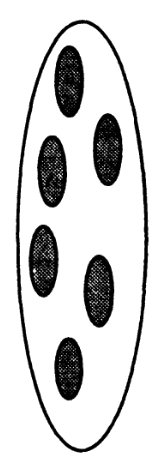
\includegraphics[height=150pt]{pictures/partons}
            \end{figure}
        \end{column}
    \end{columns}

    \footnotetext{The actual structure of the proton has a non-perturbative
    origin, so it cannot be completely understood by perturbative QFT} 
\end{frame}


\begin{frame}{LO PDF definition}
    \begin{columns}
        \begin{column}{0.55\textwidth}
            Since they are free the main property of each parton is the
            fraction of the total momentum it carries.\newline

            The probability distribution of finding a parton $p$ with momentum
            fraction $x$ it's encoded in its \textit{Parton Density Function}\footnotemark,
            $f_p(x)$.
        \end{column}
        \begin{column}{0.45\textwidth}
            Plot LO PDFs 

            %\begin{figure}
                %\centering
                %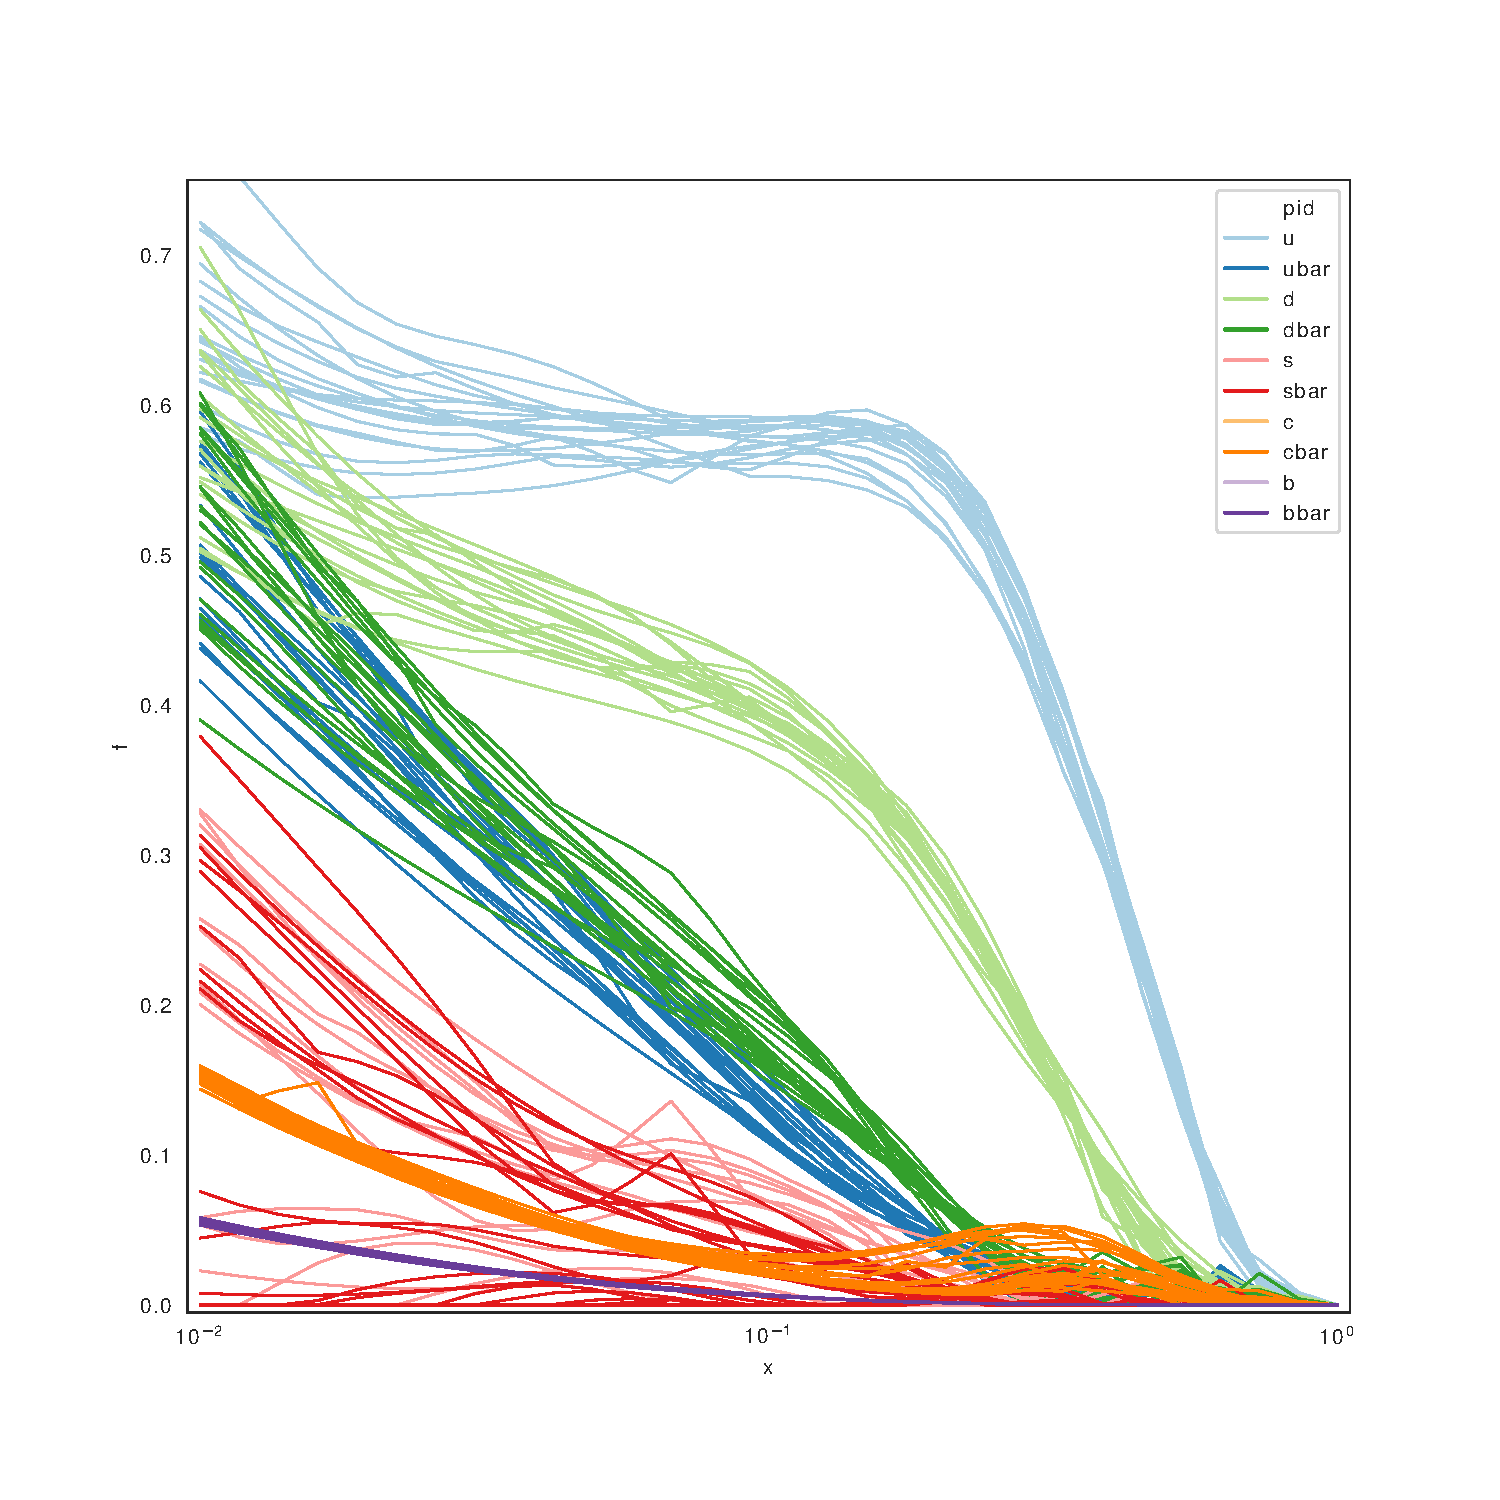
\includegraphics[height=150pt]{pictures/lo_pdfs}
            %\end{figure}
        \end{column}
    \end{columns}
    \footnotetext{In general PDFs also depend on the energy scale $Q^2$, but at
    LO they scale (see \textit{Björken scaling}). This statement can be
    explained by perturbative QCD and systematically improve, including the
    dependency through $\alpha_s$.}
\end{frame}

\section{PDF @ NLO: factorization scheme}
\begin{frame}{NLO divergences}
    As well known at NLO divergences start to appear, both in virtual and real contributions. 
    \begin{figure}
        \centering
        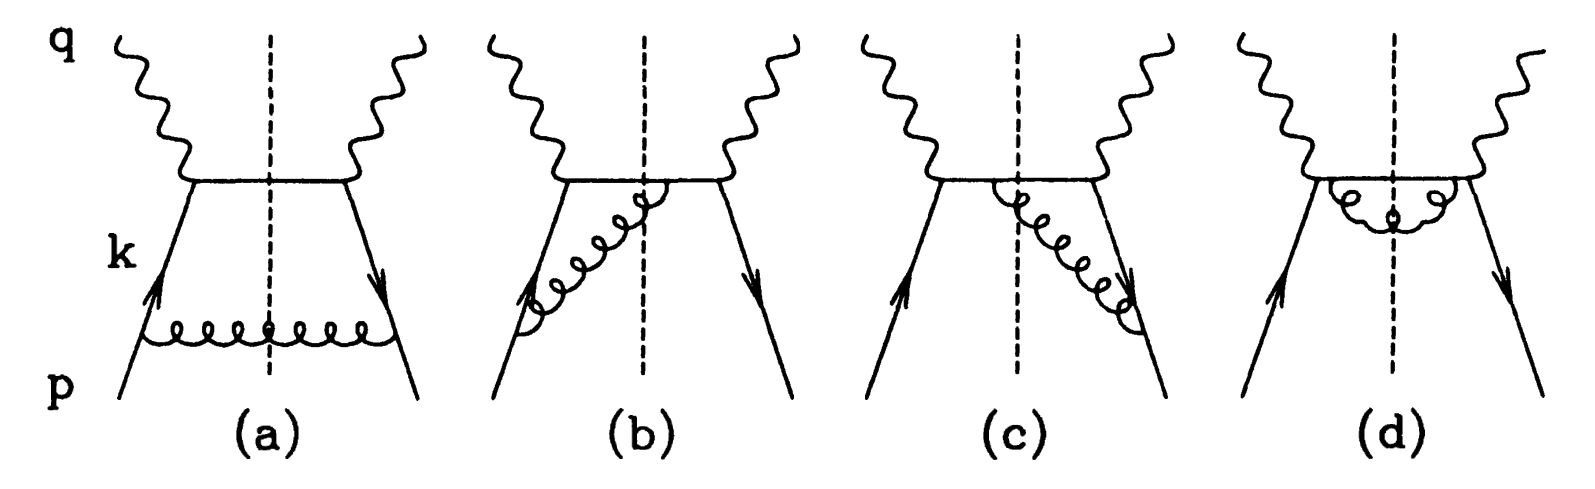
\includegraphics[width=.8\textwidth]{pictures/nlo-real}
    \end{figure}
    There are 3 kinds of divergences:
    \begin{itemize}
        \item \textbf{virtual}, due to loop integrals
        \item \textbf{soft}, due to emission of an extra soft particle
        \item \textbf{collinear}, due to 
    \end{itemize}
    The first two kinds are known to cancel in sufficiently inclusive
    observables\footnote{e.g.: the KLN theorem is one of the results that guarantee
    this cancellation.}.
\end{frame}

\begin{frame}{NLO collinear divergences}
    On the other hand collinear divergences have \textit{a different origin}
    that can be related to the asymptotic freedom of strong interactions:
    
    \begin{center}
        \textit{The collinear limit corresponds to a long range (soft) part of
        the strong interaction, which is not calculable in perturbation
        theory.}
    \end{center}

    These divergences must be treated in a different way, defining a suitable
    \textbf{factorization scheme}.\newline

    Notice that collinear divergences are also responsible for the appearance
    of the characteristic $\alpha_s \log(Q^2)$, that will introduce the PDF
    dependency on $Q^2$.
\end{frame}
    
\begin{frame}{Factorization Scheme}
    \vspace*{15pt}
    The way to deal with these divergences is offered by the previous
    interpretation: we can hide them in a non-perturbative object, the PDF.
    \begin{align*}
        F_2(x,Q^2) &= x\sum_{q,\bar{q}} q_0 \otimes \hat{F}_{2,0} (x, Q^2) =
        x \sum_{q,\bar{q}} \int\limits_x^1 \frac{\dd\xi}{\xi} q_0(\xi)
        \hat{F}_{2,0}\left(\frac{x}{\xi},Q^2\right)\\
        &= x \sum_{q,\bar{q}} q \otimes \hat{F}_2 (x, Q^2)\\
    \end{align*}
    \vspace*{-15pt}

    Example: DIS scheme for DIS @ NLO
    \begin{align*}
        \hat{F}_{2,0}(x,Q^2) &= e_q^2 x \left[ \delta(1-x) +
        \frac{\alpha_s}{2\pi}\left(P(x) \log(\frac{Q^2}{\kappa^2}) +
        C(x)\right) + \dots \right]\\
        q(x, \mu^2_F) &= q_0(x) + \frac{\alpha_s}{2\pi} \int\limits_x^1
        \frac{\dd \xi}{\xi} q_0(\xi) \left\{ P\left(\frac{x}{\xi}\right)
        \log(\frac{\mu^2_F}{\kappa^2}) + C\left(\frac{x}{\xi}\right)\right\} +
        \dots
    \end{align*}
\end{frame}

\begin{frame}{Factorization Scheme}
    This will result:
    \begin{itemize}
        \item in the effective \textit{subtraction} of the collinear divergence
            in the partonic cross section
        \item the definition of a "renormalized" PDF
        \item the appearance of a new unphysical energy scale: $\mu_F$, the
            \textit{factorization scale} (which is on the same ground of $\mu_R$).
    \end{itemize}

    There is an \textbf{arbitrariness} on defining the finite part of the
    subtraction, in the very same way of the renormalization scheme. 

    However, since the subtraction is related to a redefinition of the PDFs,
    once that a scheme has been \textbf{chosen} (fixing a finite subtraction)
    it should be kept for all the processes, because the \textbf{PDFs are
    always the same}.
\end{frame}

\begin{frame}{Factorization Scheme (CS counterterm)}
    The formula for a cross section in a generic factorization scheme can be
    written as an additional counterterm contribution $\dd\sigma^C_a$, in this
    case coming from the PDF redefinition:
    \begin{align*}
        \sigma_a^{NLO}(p; \mu_F^2) &= \int\limits_{m+1} \dd\sigma^R_a(p) +
        \int\limits_{m} \dd\sigma^V_a(p) + \int\limits_{m} \dd\sigma^C_a(p;
        \mu_F^2)\\
        \dd\sigma^C_a(p;\mu_F^2) &= - \frac{\alpha_s}{2\pi}
        \frac{1}{\Gamma(1-\epsilon)} \sum_b \int\limits_0^1 \dd z \left[ -
        \frac{1}{\epsilon} \left(\frac{4\pi\mu^2}{\mu_F^2}\right)^\epsilon
        P^{ab}(z) + K^{ab}(z) \right] \dd \sigma_b^B(zp) 
    \end{align*}
    in dimensional regularization\footnote{The counterterm is such that
    $K^{ab}=0$ for $\msbar$ factorization scheme}.

    This will be useful in what follows, because it is exactly by choosing a
    specific factorization scheme (i.e. a specific $K^{ab}$ matrix) that we can
    analyze the property of the frequent $\msbar$ choice.
\end{frame}

\section{An intrinsic positive scheme}
\begin{frame}{Is there a positive scheme?}
    At LO PDFs are positive by construction, since they are defined as
    probability distributions, but this is not true at NLO, since we redefined
    the PDF with the subtraction from the factorization scheme.\newline

    So the question:

    \begin{center}
        \textit{Does it exist at all a factorization scheme in which PDF are\\ still positive also @ NLO?}
    \end{center}

    And the answer can be ready given: \textbf{Yes}.\newline 

    It results that there is not a single positive scheme, but there is a special class of them.
\end{frame}

\begin{frame}{A physical scheme}
    A special class of factorization scheme is the one in which the PDFs are
    directly defined on \textbf{physical observables}, subtracting \textit{all
    of the finite} contribution. 

    Like in the DIS scheme we can choose two physical processes for defining the quark and gluon PDF:
    \begin{description}
        \item[quark] we can choose a hypothetical $\bar{q} p \to \gamma^* + X$
        (Drell-Yan with a pure antiquark beam), or a DIS structure function; 
        \item[gluon] either a hypothetical $g p \to H + X$ (gluon fusion with a
        pure gluon beam), or a photon-gluon fusion;
    \end{description}
\end{frame}

\begin{frame}{The $\phys$ scheme}
    We can choose one of these schemes and call it $\phys$, for example:
    \begin{align*}
        \frac{1}{x}\bar{\sigma}(x,Q^2) &= f^{\,\phys}(x,Q^2)\\ 
        \bar{\sigma}(x,Q^2) &= \begin{pmatrix} 
        \sigma(x,Q^2)[\bar{q} p \to \gamma^* + X]\\
        \sigma(x,Q^2)[g p \to H + X]
        \end{pmatrix}
    \end{align*}

    As one can deduce from the first equation this scheme is positive by
    construction, since the PDF is proportional to a physical cross-section,
    whose positivity is guaranteed.
\end{frame}

\section{Coefficient functions NLO behaviour}
\begin{frame}{Universality of collinear structure}
    We can play this game because we know in advance that the relevant structure (the one related to the collinear subtraction) is universal.
\end{frame}

\begin{frame}{Scheme change matrix}
    How we switch scheme and $K$ properties
\end{frame}

\begin{frame}{A bunch of nontrivial positivity schemes}
    POS, MPOS, DPOS
\end{frame}

\section{Is $\msbar$ negative?}
\begin{frame}{Introduction}
    Argument from MPOS -> MSbar
\end{frame}

\section{Why positivity?}
\begin{frame}{My opinion?}
    Reduce PDF variance limiting the hypothesis space. 
\end{frame}


\begin{frame}[standout]
    Thanks for your attention
\end{frame}

\appendix

\begin{frame}{N-space positivity $\neq$ x-space positivity}
    The easy way in \textit{N-space} and Why we need an argument in \textit{x-space}
\end{frame}

\begin{frame}{NLL calculation}
    The calculation in $x \to 1$ limit, better not to include in the main body (eq. 50-53)
\end{frame}

\begin{frame}{Heavy quarks}
    Spend some words on heavy quarks' schemes and how the proof extend.
\end{frame}


\end{document}
